% =============================================================================
% Paper A -- Target: Applied Mathematics in Science and Engineering / IEEE Transactions
% =============================================================================
\documentclass[11pt,a4paper]{article}

\usepackage[utf8]{inputenc}
\usepackage[T1]{fontenc}
\usepackage{geometry}
\geometry{top=1in, bottom=1in, left=1in, right=1in}
\usepackage{amsmath}
\usepackage{amssymb}
\usepackage{microtype}
\usepackage{graphicx}
\usepackage{booktabs}
\usepackage{multirow}
\usepackage{xcolor}
\usepackage{hyperref}
\usepackage{cite}

\graphicspath{{figures/}}

\hypersetup{
    colorlinks=true,
    linkcolor=blue,
    filecolor=magenta,
    urlcolor=cyan,
    citecolor=blue,
}

\title{\textbf{Self-Supervised Contrastive Anomaly Detection in Power-Converter Frequency-Response Signatures}}

\author{
    \textbf{Ignacio Martin-Salinas}, \textbf{Jose A. Belloch}, \textbf{Adri{\'a}n Amor-Mart{\'\i}n}, \textbf{Pablo Zumel}, \textbf{Cristina Fernandez} \\
    \small Department of Electronic Technology, Universidad Carlos III de Madrid, 28911 Legan{\'e}s, Madrid, Spain
}
\date{}

\begin{document}
\maketitle

\begin{abstract}
Component degradation in power electronic converters (PECs) precedes catastrophic electrical failure through subtle, non-linear parametric drift that conventional fixed-threshold scalar alarms fail to resolve. This paper presents a self-supervised anomaly detection framework operating directly on the converter's frequency-domain transfer-function (Bode) signature. We adapt the synthetic-negative principle of Contrastive Representation Learning for Anomaly Detection (CARLA) into a contrastive autoencoder equipped with a \emph{physics-informed negative sampler}. Rather than perturbing signatures using domain-agnostic heuristics, candidate negative samples are synthesized from the analytic complex transfer ratio between nominal and component-perturbed small-signal converter models. Multiplying an observed healthy response by this ratio generates hard negative samples whose magnitude and phase evolve coherently under governing circuit laws. We formalize the anomaly classification problem as a set-membership rule over component-specific multiplier bands derived from manufacturing tolerances and degradation literature. A Latin Hypercube Sampling (LHS) strategy is implemented to generate both healthy operating envelopes and multi-fault degradation regimes. We benchmark five neural encoder families---One-Dimensional Convolutional Neural Networks (Conv1D), Long Short-Term Memory (LSTM), Gated Recurrent Units (GRU), Multi-Layer Perceptrons (MLP), and Multi-Head Self-Attention Transformers---under a unified hyperparameter optimization and non-parametric $k$-nearest-neighbor ($k$-NN) scoring protocol. On a held-out test set of 1,268 physically distinct converter states (520 healthy and 748 anomalous), Conv1D achieves the highest F1-score (0.8897) and Precision-Recall Area Under Curve (PR-AUC, 0.9570), while MLP attains the highest Receiver Operating Characteristic Area Under Curve (ROC-AUC, 0.9161). In a paired ablation across three independent random initializations with byte-identical starting weights, physics-informed synthesis improves mean F1 from $0.8659\pm0.0154$ to $0.8840\pm0.0054$ (paired $\Delta$ $+0.0181$, individual deltas $+0.0366$, $-0.0038$, $+0.0215$). With $n=3$ the effect is descriptive; formal significance testing is underpowered and therefore omitted in favor of effect size and per-seed reporting.
\end{abstract}

\noindent\textbf{Keywords:} Anomaly Detection; Power Electronics; Self-Supervised Learning; Contrastive Representation Learning; Autoencoders; Transfer Function; Physics-Informed Machine Learning

\section{Introduction}
\label{sec:intro}

Power electronic converters (PECs) serve as critical energy-processing infrastructure across aerospace platforms, electric vehicles, industrial drives, and renewable-dominated power grids~\cite{idrisov2025digitaltwin}. In these mission-critical applications, component-level degradation---such as output filter capacitor electrolyte loss and dielectric wear-out, inductor core thermal degradation and saturation, and power MOSFET on-state resistance drift---develops gradually and non-linearly over extended operating cycles~\cite{celaya2011mosfet,kulkarni2010electrolytic,dang2020capacitors}. Because these parametric drifts precede outright catastrophic short- or open-circuit failure by a substantial operational window, early-stage detection is essential for condition-based predictive maintenance. Conventional supervisory systems rely predominantly on manual inspection routines or static threshold alarms on scalar variables (e.g., peak output voltage, average current, or discrete temperature thresholds). However, scalar indicators are fundamentally insensitive to joint, multi-component degradation profiles and fail to detect incipient parametric anomalies that remain within nominal steady-state operating limits~\cite{liu2023review,kou2023faultdiagnosis}.

Data-driven anomaly detection offers a compelling paradigm: rather than engineering hand-crafted fault rules for every conceivable degradation mode, an algorithm learns the underlying manifold of \emph{healthy} operating signatures and flags statistically significant deviations~\cite{beattie2022robust,gomez2024selfcommissioning}. Despite recent advances in deep time-series anomaly detection, two major obstacles persist in power electronics:
\begin{enumerate}
    \item \textbf{Label Scarcity and Asymmetry:} True operational fault data is scarce, hazardous, and expensive to capture in physical plants. Consequently, high-fidelity physics-based digital twins must provide the nominal and degraded state space, and training gradients must rely strictly on healthy observations without supervising on fault labels.
    \item \textbf{Representation Collapse in Contrastive Learning:} Contrastive representation learning optimizes an encoder to cluster representations of similar views while repelling dissimilar views~\cite{chen2020simclr}. In an unsupervised anomaly detection setting where training distributions contain exclusively healthy observations, drawing negative pairs from within the mini-batch repels valid nominal states, degrading latent topology. Conversely, avoiding negative mining altogether risks trivial representation collapse~\cite{chen2023harnessing,zhang2025encodethendecompose}. The CARLA framework~\cite{darban2025carla} resolves this dilemma by computationally \emph{synthesizing} negative instances. However, conventional negative-synthesis operators (such as Gaussian spectral noise, random time warping, and scalar amplitude scaling) are domain-agnostic heuristics that violate fundamental circuit principles, producing unphysical spectral signatures that do not reflect realistic degradation dynamics.
\end{enumerate}

To overcome these limitations, this paper introduces a \textbf{physics-informed negative sampler} for self-supervised contrastive anomaly detection on converter frequency-response (Bode) signatures. The foundational scientific insight is that for linear time-invariant (LTI) or linearized dynamical systems, the transition between nominal and degraded physical states is an analytically tractable, multiplicative complex operator in the Laplace domain. Rather than applying heuristic signal corruptions that violate circuit laws, candidate negative samples are synthesized by evaluating the analytical transfer ratio between nominal and component-perturbed small-signal models. Multiplying the observed healthy response by this ratio generates hard negative instances where magnitude and phase evolve coherently under governing differential equations. This resolves the one-class contrastive dilemma: it replaces isotropic, unphysical noise with an \emph{anisotropic manifold regularizer} that directs contrastive repulsive gradients exclusively along genuine physical degradation hyperplanes.

The specific scientific and methodological contributions of this work are as follows:
\begin{enumerate}
    \item \textbf{Analytic Transfer-Ratio Generative Principle:} We establish a zero-ODE-overhead generative operator for contrastive learning in physical dynamical systems: multiplying observed frequency signatures by analytic transfer ratios $\tilde{H}(s)/H^{(0)}(s)$ generates hard negatives that preserve pole-zero structure and coherent magnitude-phase warps without numerical integration (Section~\ref{sec:carla}). Under the small-signal linear time-invariant (LTI) assumption, the operator preserves analyticity in $\mathbb{C}$ and avoids per-sample differential-equation solves.
    \item \textbf{Resolution of the One-Class Contrastive Dilemma:} We formulate a directed, two-logit InfoNCE objective that avoids intra-manifold false-negative repulsion of healthy states while constructing an anisotropic repulsive barrier along continuous component degradation trajectories (Section~\ref{sec:carla}).
    \item \textbf{Formal Set-Membership Formulation:} We formalize the anomaly classification problem on power-converter transfer functions as an explicit set-membership rule over component-wise parameter multiplier bands derived from manufacturing tolerances and degradation literature (Section~\ref{sec:problem}).
    \item \textbf{Physics-Aware Sampling Protocol:} We implement a Latin Hypercube Sampling (LHS) methodology to construct both a continuous healthy tolerance envelope and a multi-fault regime combining primary faults with independently triggered secondary parametric variations (Section~\ref{sec:dataset}).
    \item \textbf{Systematic Encoder Benchmarking and Inductive Bias Analysis:} We conduct a comprehensive empirical evaluation of five distinct encoder families (Conv1D, LSTM, GRU, MLP, and Transformer), mathematically characterizing why coordinate-aware feedforward and convolutional models outperform sequential recurrent architectures on discrete logarithmic frequency grids (Sections~\ref{sec:baselines} and~\ref{sec:results}).
    \item \textbf{Controlled Statistical Ablation:} We perform a paired, weight-hash-verified ablation across multiple independent random initializations to isolate the quantitative gain of physics-informed negative synthesis over domain-agnostic heuristics (Section~\ref{sec:results}).
\end{enumerate}

A companion study~\cite{jsc_edge_deployment} investigates the systems-level computational optimization, operator lowering, and embedded GPU deployment of these trained architectures on edge computing hardware (NVIDIA Jetson Nano). This paper focuses on the mathematical formulation, representation learning framework, and diagnostic evaluation.

\section{Related Work}
\label{sec:related}

\subsection{Autoencoder-Based Anomaly Detection}
Reconstruction-based anomaly detection trains a neural autoencoder to reconstruct nominal operating signatures, using the resulting reconstruction error as an anomaly score. Foundational feedforward architectures~\cite{rumelhart1986backprop} have been extended to recurrent networks utilizing LSTM~\cite{hochreiter1997lstm} and GRU~\cite{cho2014gru} cells for sequential dependencies, One-Dimensional Convolutional Neural Networks (Conv1D)~\cite{kiranyaz2019survey} for local correlation extraction across frequency bands, Multi-Head Self-Attention Transformers~\cite{vaswani2017attention} for global receptive fields, and Variational Autoencoders (VAEs)~\cite{kingma2013autoencoding} that constrain the latent space with a Kullback--Leibler (KL) divergence prior. 

However, purely reconstruction-based objectives penalize only deviations from the nominal training distribution without explicitly structuring the latent space for discriminative separation. This limitation has motivated hybrid contrastive-reconstruction models~\cite{gao2020robusttad,campos2021unsupervised,zimmerer2018contextvae} and heightened scrutiny regarding evaluation methodologies~\cite{yuan2022trustworthy}. Notably, Kim et al.~\cite{kim2021towards} demonstrated that point-adjustment heuristics common in time-series benchmarks artificially inflate F1-scores and distort model rankings. In this study, all evaluations are conducted at the individual sample level without point adjustment, reporting both threshold-dependent metrics (F1, precision, recall) and threshold-independent ranking metrics (ROC-AUC~\cite{fawcett2006roc}, PR-AUC).

\subsection{Contrastive and Self-Supervised Learning}
Contrastive learning trains neural feature extractors by maximizing mutual information between positive views of an instance while minimizing agreement with negative views via objectives such as InfoNCE or NT-Xent~\cite{oord2018representation,chen2020simclr}. Adapting contrastive learning to unsupervised anomaly detection is challenging because true anomalous states are unavailable during training. To avoid representation collapse when sampling negatives from an exclusively normal pool~\cite{chen2023harnessing}, CARLA~\cite{darban2025carla} constructs synthetic negatives through signal-processing heuristics (e.g., uniform noise, spectral masking, and temporal warping). 

Recent developments emphasize the importance of domain-consistent augmentations. DCdetector~\cite{yang2023dcdetector} employs a dual-attention architecture to learn permutation-invariant representations without explicit negatives. Kim et al.~\cite{kim2025causalityaware} utilize causal discovery to separate normal variations from structure-breaking anomalies. Similarly, physics-informed generative and diffusion models demonstrate that embedding governing physical constraints yields superior density estimation and anomaly discrimination~\cite{raissi2019pinn,soni2025physicsinformed}. Our framework instantiates this domain-grounded principle directly: rather than training a separate generative network, it applies the analytic small-signal transfer ratio of the physical plant to synthesize hard negatives in real time.

\subsection{Data-Driven Fault Diagnosis in Power Electronics}
Machine learning for PEC diagnostics has evolved from shallow classifiers operating on wavelet-transformed features~\cite{kou2023faultdiagnosis} to deep neural architectures, explainable AI pipelines~\cite{beattie2022robust,li2025explainability}, and digital-twin-assisted condition monitoring~\cite{idrisov2025digitaltwin,gomez2024selfcommissioning}. Extensive surveys categorize both open-circuit switch faults and gradual parametric degradation in passive components~\cite{liu2023review,dang2020capacitors}. While existing works largely treat fault detection as either a supervised classification task or an unconstrained time-series problem, this paper grounds both the dataset labeling rule and the contrastive pretext task in the governing small-signal physics of the converter.

\section{Problem Formulation}
\label{sec:problem}
This section develops the applied mathematical foundation: the governing linear differential equations of the converter, their Laplace-domain boundary-value representation, stability of the resulting second-order system, and the set-membership formalization that grounds anomaly labels in manufacturing tolerances. The formulation connects circuit-level differential dynamics to a discrete frequency-domain inverse problem amenable to computational learning.

\begin{figure}[t]
\centering
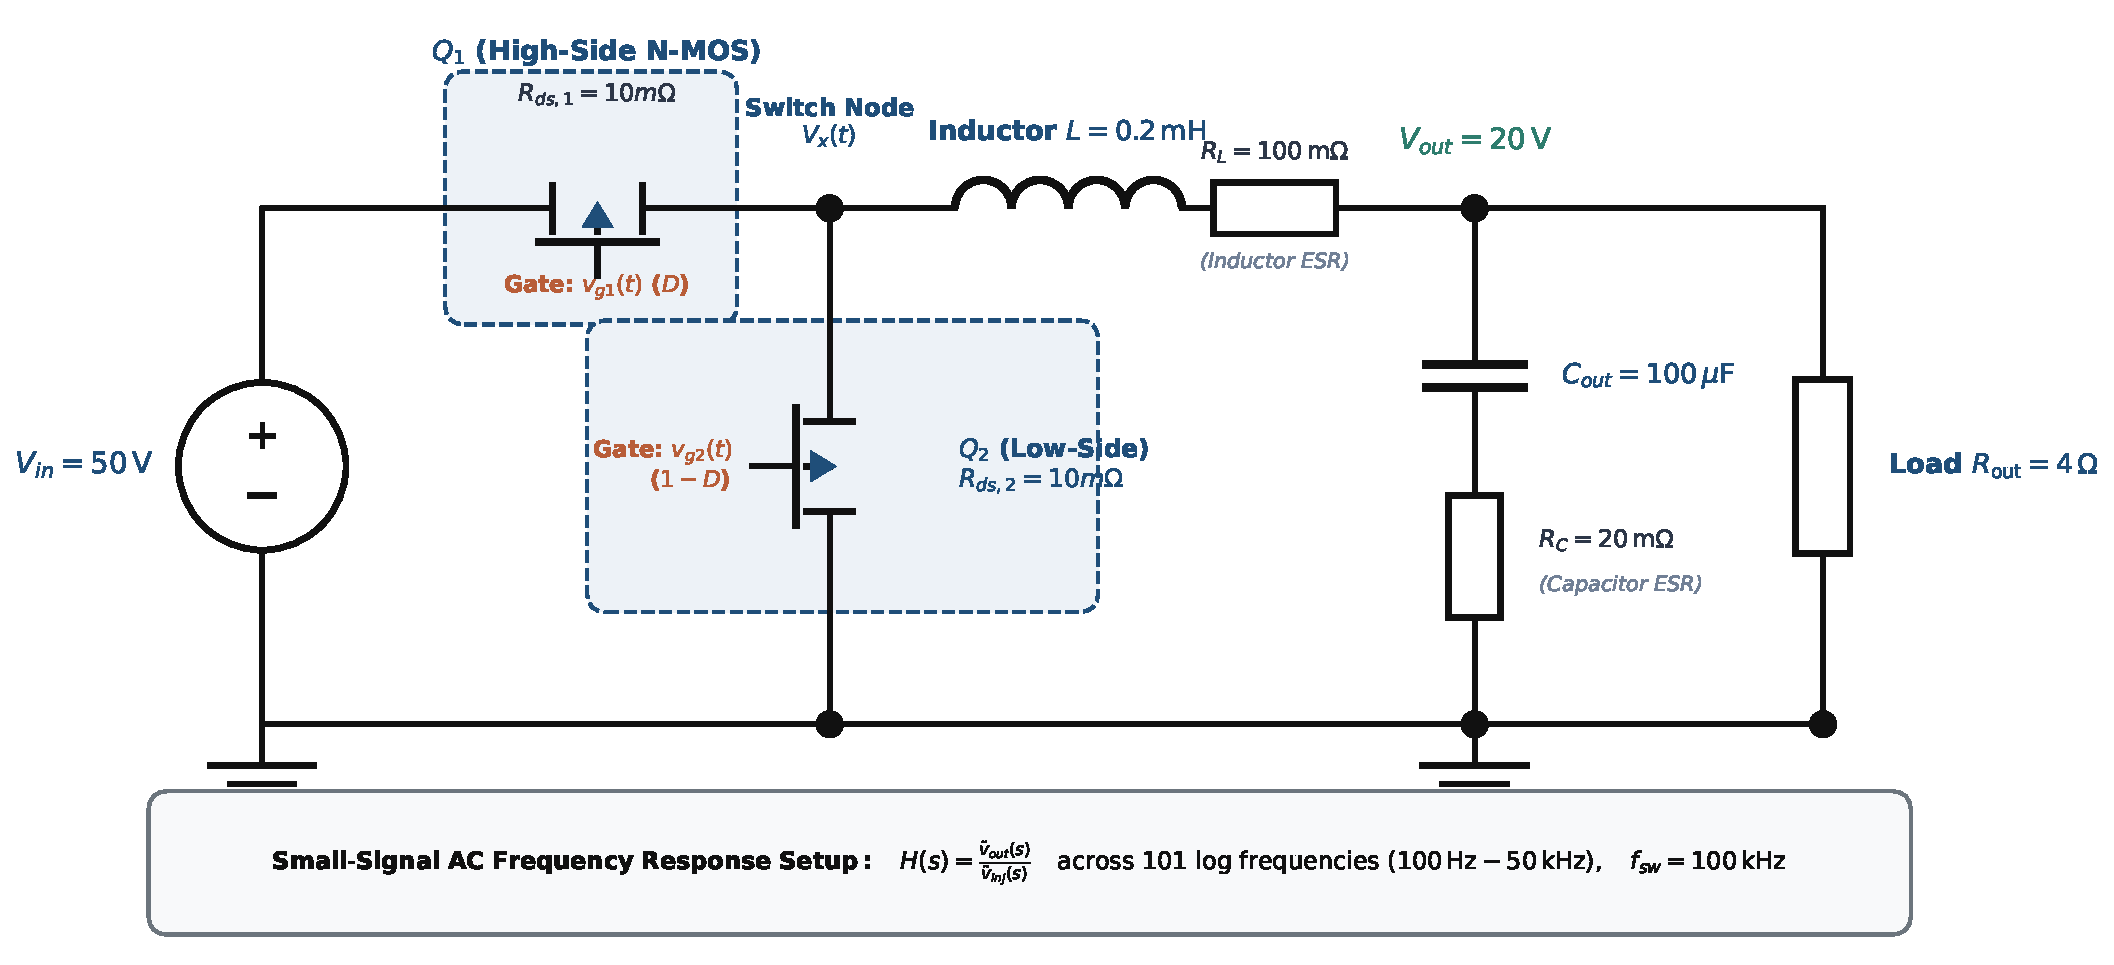
\includegraphics[width=0.88\textwidth]{buck_converter_schematic.pdf}
\caption{Synchronous Buck converter topology serving as the reference power plant. Baseline nominal parameters: input voltage $V_{\mathrm{in}}=50\text{ V}$, output voltage $V_{\mathrm{out}}=20\text{ V}$, filter inductance $L=0.2\text{ mH}$, output capacitance $C_{\mathrm{out}}=100\ \mu\text{F}$, inductor winding resistance $R_{\mathrm{ESR},L}=100\ \text{m}\Omega$, capacitor equivalent series resistance $R_{\mathrm{ESR},C}=20\ \text{m}\Omega$, and switch on-state resistances $R_{\mathrm{ds},1}=R_{\mathrm{ds},2}=10\ \text{m}\Omega$.}
\label{fig:buck-schematic}
\end{figure}

We consider a synchronous buck converter plant (Fig.~\ref{fig:buck-schematic}) operating in continuous conduction mode (CCM) under voltage-mode control with fixed switching frequency $f_{s}=100\,\text{kHz}$ (see CCM bound below). The health status of the converter is captured by its small-signal duty-cycle-to-output-voltage transfer function
\begin{equation}
G_{vd}(s) = \frac{\hat{v}_{\mathrm{out}}(s)}{\hat{d}(s)}\,,
\label{eq:gvd-def}
\end{equation}
where $\hat{v}_{\mathrm{out}}(s)$ and $\hat{d}(s)$ represent Laplace-domain perturbations in output voltage and duty ratio, respectively. Applying state-space averaging~\cite{erickson2001fundamentals}, $G_{vd}(s)$ is expressed in canonical second-order form as:
\begin{equation}
G_{vd}(s) = V_{\mathrm{in}} \frac{1 + s/\omega_z}{1 + \dfrac{s}{Q\omega_0} + \left(\dfrac{s}{\omega_0}\right)^2}\,,
\label{eq:gvd}
\end{equation}
with the characteristic undamped natural angular frequency $\omega_0$, equivalent series resistance (ESR) zero angular frequency $\omega_z$, and quality factor $Q$ defined by:
\begin{equation}
\omega_0 = \frac{1}{\sqrt{L C_{\mathrm{out}}}}\,, \qquad
\omega_z = \frac{1}{R_{\mathrm{ESR},C} C_{\mathrm{out}}}\,,
\label{eq:corner-freqs-w}
\end{equation}
\begin{equation}
\frac{1}{Q} = \frac{\omega_0 L}{R_{\mathrm{out}}} + \omega_0 C_{\mathrm{out}} R_{\mathrm{ESR},C} + \frac{R_{\mathrm{ESR},L} + R_{\mathrm{ds},\mathrm{eff}}}{\omega_0 L}\,.
\label{eq:quality-factor}
\end{equation}
In Eq.~\eqref{eq:quality-factor}, $R_{\mathrm{ds},\mathrm{eff}} = D R_{\mathrm{ds},1} + (1-D) R_{\mathrm{ds},2}$ denotes the duty-cycle-weighted conducting-path resistance of the primary and synchronous MOSFET switches, where $D = V_{\mathrm{out}}/V_{\mathrm{in}} = 0.40$ represents the steady-state nominal duty cycle under voltage-mode continuous conduction regulation ($V_{\mathrm{in}}=50\text{ V}, V_{\mathrm{out}}=20\text{ V}$) and nominal load $R_{\mathrm{out}}^{(0)}=4\,\Omega$ (Fig.~\ref{fig:buck-schematic}). At nominal component parameters, the resonant frequency is $f_0 = \omega_0 / (2\pi) \approx 1.125\text{ kHz}$, which lies centrally within the evaluated measurement band of $100\text{ Hz}$ to $50\text{ kHz}$. The ESR zero frequency $f_z = \omega_z / (2\pi) \approx 79.58\text{ kHz}$ resides beyond the upper sweep boundary under nominal conditions, shifting into the active measurement band only under severe capacitor degradation. For all admissible $\boldsymbol{\theta}$, $\mathrm{Re}\{p_i\}<0$ so the second-order plant remains strictly stable (Hurwitz); degradation shifts damping $Q^{-1}$ but preserves open-loop stability under the CCM bound below.

\subsection{Continuous Conduction Mode (CCM) Validity and Stability Bounds}
The second-order transfer function in Eq.~\eqref{eq:gvd} — the Laplace transform of the averaged inductor-current and capacitor-voltage linear differential equations — holds strictly when the converter operates in CCM. Stability follows from the denominator $1+s/(Q\omega_{0})+(s/\omega_{0})^{2}$ with $Q>0$, $\omega_{0}>0$: the poles $p_{1,2}=-\omega_{0}/(2Q)\pm j\omega_{0}\sqrt{1-1/(4Q^{2})}$ satisfy $\mathrm{Re}\{p_{i}\}<0$ for all admissible $\boldsymbol{\theta}$, so the open-loop plant is Hurwitz-stable and degradation only modulates damping and resonance. Under the fixed switching frequency $f_{s}=100\,\text{kHz}$, the boundary condition guaranteeing CCM operation across the continuous parameter state space is:
\begin{equation}
L > L_{\mathrm{crit}} = \frac{(1 - D) R_{\mathrm{out}}}{2 f_s}\,.
\label{eq:ccm-bound}
\end{equation}
Under nominal load resistance $R_{\mathrm{out}}^{(0)} = 4\ \Omega$, the critical inductance is $L_{\mathrm{crit}} = \frac{(1 - 0.40) \cdot 4\ \Omega}{2 \cdot 100\times 10^3\text{ Hz}} = 12\ \mu\text{H}$. Even under light-load variations up to $R_{\mathrm{out}} = 20\ \Omega$ ($5\times R_{\mathrm{out}}^{(0)}$), the critical inductance remains $L_{\mathrm{crit}} = 60\ \mu\text{H}$. Given the lowest boundary of degraded filter inductance in the fault band ($m_L = 0.40 \implies L_{\mathrm{min}} = 80\ \mu\text{H}$), the condition $L_{\mathrm{min}} > L_{\mathrm{crit}}$ is strictly satisfied with a deterministic margin across all operating regimes ($L_{\mathrm{min}} \ge 1.33 \times L_{\mathrm{crit}}$ under light load, and $L_{\mathrm{min}} = 6.67 \times L_{\mathrm{crit}}$ under nominal load). Across operating load variations $R_{\mathrm{out}} \in [0.50, 2.00]\times R_{\mathrm{out}}^{(0)}$, the converter remains strictly in second-order CCM dynamics, preventing discontinuous conduction mode (DCM) transitions from reducing the dynamic system order.

\subsection{Parametric Degradation as Component Multipliers}
Let $\boldsymbol{\theta} = [C_{\mathrm{out}}, L, R_{\mathrm{ds},1}, R_{\mathrm{ds},2}, R_{\mathrm{ESR},C}, R_{\mathrm{ESR},L}]^\top \in \mathbb{R}^6$ denote the vector of degradable physical parameters, with nominal baseline $\boldsymbol{\theta}^{(0)}$. We define the non-dimensional multiplier vector $\mathbf{m} = \boldsymbol{\theta} \oslash \boldsymbol{\theta}^{(0)}$ through element-wise division, such that $\mathbf{m} = \mathbf{1}$ represents the nominal operating point. 

Each component $i$ is assigned a \emph{normal} multiplier tolerance band $\mathcal{M}_i^n \subset \mathbb{R}^+$ and a disjoint \emph{anomalous} degradation band $\mathcal{M}_i^a \subset \mathbb{R}^+$. These intervals are defined according to industrial component tolerance standards (e.g., IEC 60384-1 generic capacitor specifications~\cite{iec60384_1}, DC-bias derating characteristics~\cite{waugh_dcbias}) and accelerated aging literature~\cite{celaya2011mosfet,kulkarni2010electrolytic,dang2020capacitors}:
\begin{itemize}
    \item Output Capacitance ($C_{\mathrm{out}}$): $\mathcal{M}_{C_{\mathrm{out}}}^n = [0.80, 1.20]$, $\mathcal{M}_{C_{\mathrm{out}}}^a = [0.30, 0.70]$.
    \item Capacitor ESR ($R_{\mathrm{ESR},C}$): $\mathcal{M}_{\mathrm{ESR},C}^n = [0.50, 2.00]$, $\mathcal{M}_{\mathrm{ESR},C}^a = [3.00, 8.00]$.
    \item Filter Inductance ($L$): $\mathcal{M}_L^n = [0.80, 1.20]$, $\mathcal{M}_L^a = [0.40, 0.70]$.
    \item Inductor ESR ($R_{\mathrm{ESR},L}$): $\mathcal{M}_{\mathrm{ESR},L}^n = [0.85, 1.40]$, $\mathcal{M}_{\mathrm{ESR},L}^a = [2.00, 6.00]$.
    \item MOSFET On-Resistances ($R_{\mathrm{ds},1}, R_{\mathrm{ds},2}$): $\mathcal{M}_{\mathrm{ds}}^n = [1.00, 2.20]$, $\mathcal{M}_{\mathrm{ds}}^a = [3.00, 15.00]$.
\end{itemize}
Load resistance $R_{\mathrm{out}}$ is swept within $[0.50, 2.00]\times$ nominal to represent healthy operating load variation; it is not assigned an anomalous fault band. The configuration is declared externally in a JSON schema, ensuring that adapting the pipeline to alternative converter topologies requires zero algorithmic modifications.

\subsection{Mathematical Labeling Rule}
A simulated converter instance characterized by multiplier vector $\mathbf{m}$ is labeled according to the set-membership rule:
\begin{equation}
y(\mathbf{m}) =
\begin{cases}
\textsf{anomalous} & \text{if } \exists\, i \in \{1,\dots,6\} : m_i \in \mathcal{M}_i^a\,, \\
\textsf{normal}    & \text{if } \forall\, i \in \{1,\dots,6\} : m_i \in \mathcal{M}_i^n\,, \\
\textsf{undefined} & \text{otherwise (excluded from training and testing).}
\end{cases}
\label{eq:label-rule}
\end{equation}

Each converter state is observed exclusively through its frequency response evaluated at $N_f = 101$ logarithmically spaced frequencies $f_k \in [100\text{ Hz}, 50\text{ kHz}]$. Magnitude (dB) and phase (degrees) responses are converted to complex Cartesian coordinates (real and imaginary components) and standardized channel-wise using mean and variance statistics fitted strictly on the healthy training subset:
\begin{equation}
\mathbf{X} = [\mathrm{Re}\{\mathbf{G}_{vd}\}_{\mathrm{norm}},\, \mathrm{Im}\{\mathbf{G}_{vd}\}_{\mathrm{norm}}] \in \mathbb{R}^{101 \times 2}\,.
\label{eq:input-tensor}
\end{equation}

\section{Dataset Generation and Computational Sampling}
\label{sec:dataset}

\begin{figure}[t]
\centering
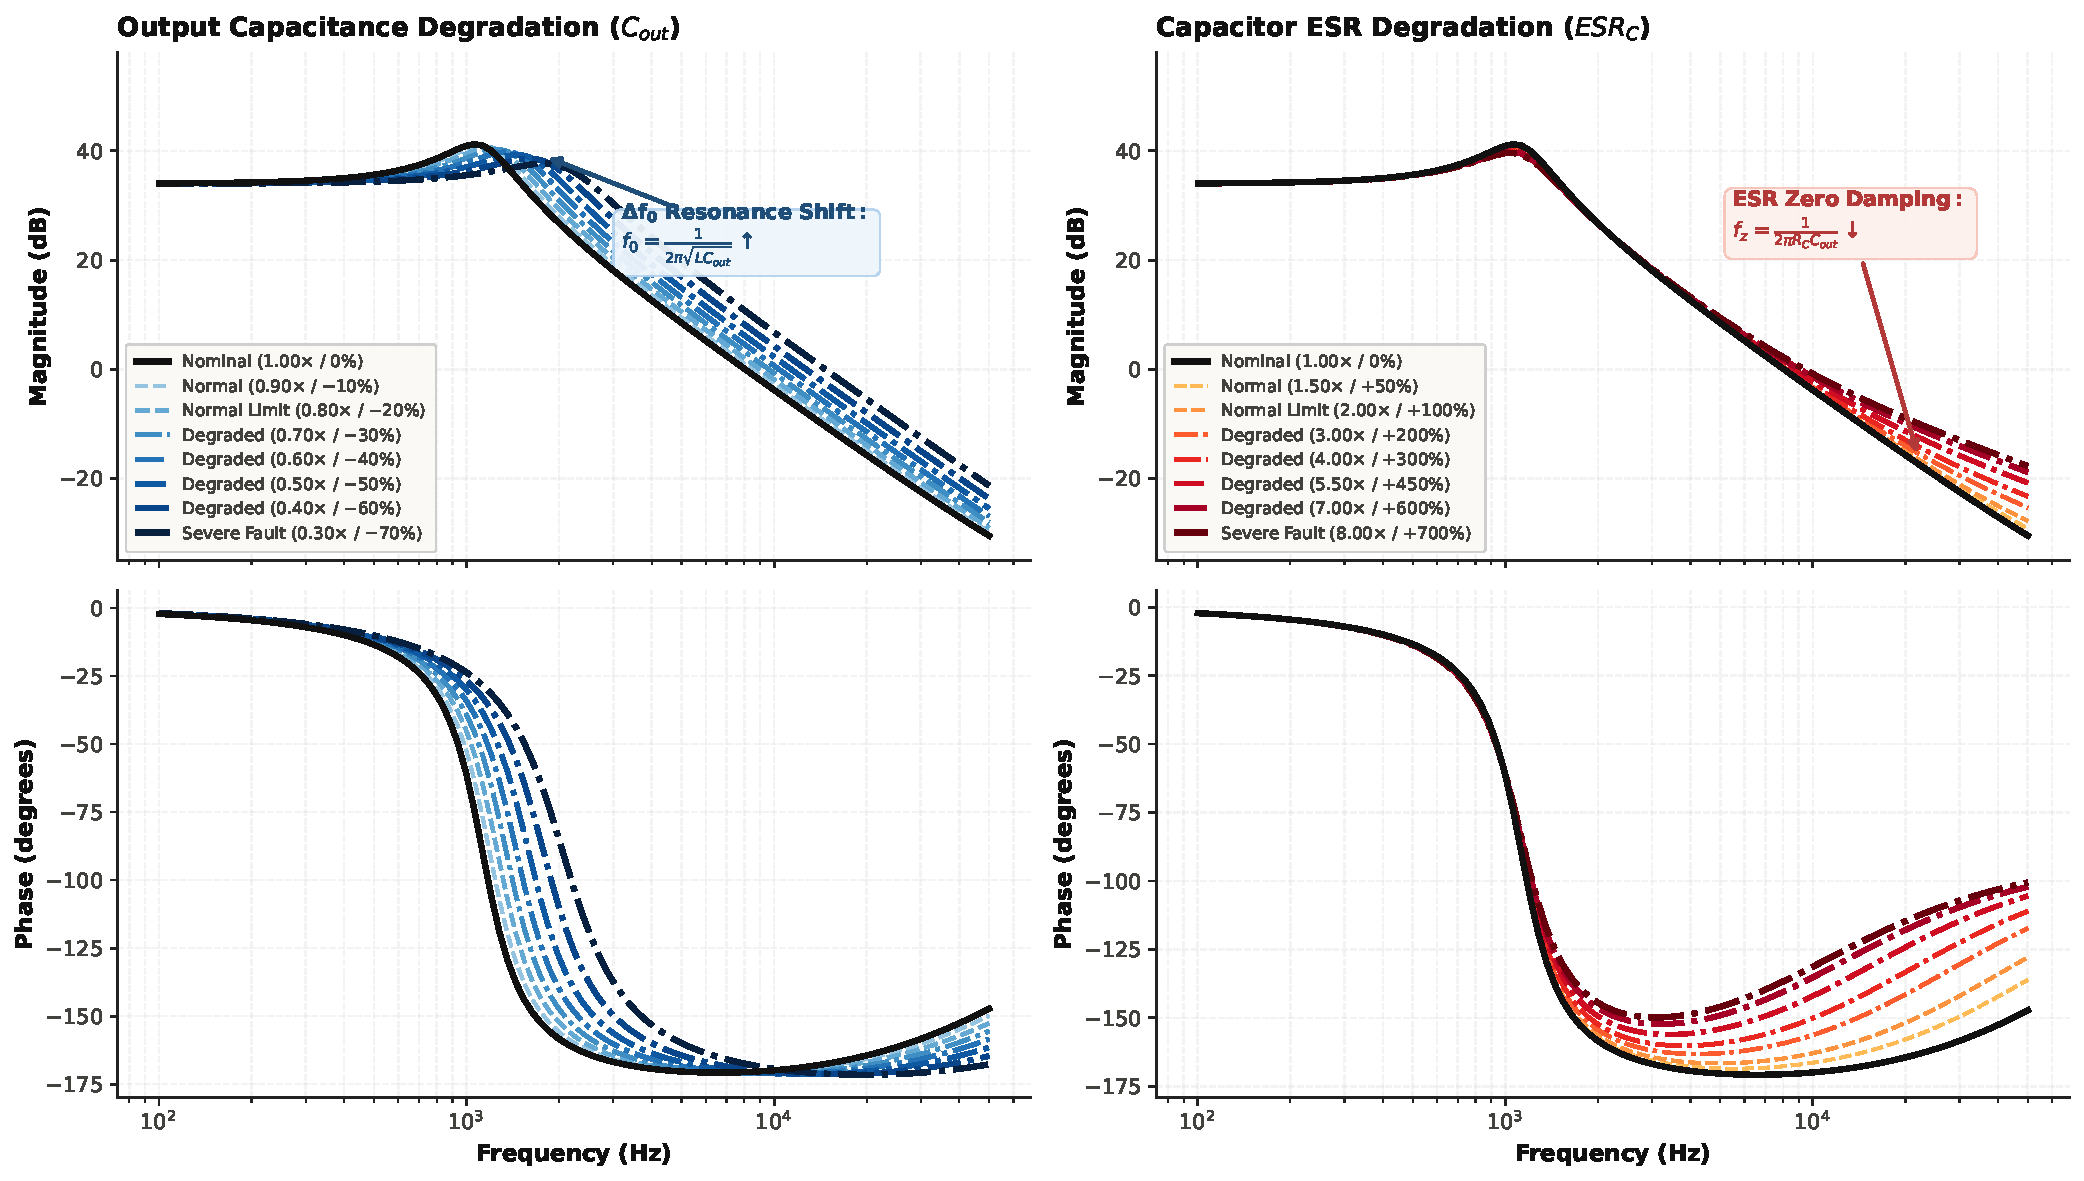
\includegraphics[width=0.95\textwidth]{component_degradation_bode.pdf}
\caption{Physical frequency-response drift under continuous component degradation across the evaluated spectrum: (left) output capacitance reduction ($C_{\mathrm{out}} \in [0.30, 1.00]\times$), inducing an upward resonance shift $\Delta f_0 \propto 1/\sqrt{L C_{\mathrm{out}}}$; (right) capacitor ESR rise ($R_{\mathrm{ESR},C} \in [1.00, 8.00]\times$), driving the ESR zero $f_z \approx 1/(2\pi R_{\mathrm{ESR},C} C_{\mathrm{out}})$ into the active measurement band.}
\label{fig:anomaly-deviation-examples}
\end{figure}

Training and evaluation data are synthesized using a high-fidelity PSIM digital twin of the synchronous buck converter (Fig.~\ref{fig:buck-schematic}), eliminating the cost, hazards, and destruction associated with physical component overstress testing. 

Two distinct sampling regimes are deployed:
\begin{itemize}
    \item \textbf{Healthy Operating Regime:} Latin Hypercube Sampling (LHS)~\cite{mckay1979comparison} is performed over the multi-dimensional bounding box $\prod_{i=1}^6 \mathcal{M}_i^n$, ensuring uniform, stratified coverage of nominal manufacturing tolerances and temperature-induced drift.
    \item \textbf{Multi-Fault Degradation Regime:} To reflect real-world aging where multiple components can degrade concurrently, each faulty instance receives one guaranteed \emph{primary} fault sampled via LHS from $\mathcal{M}_{\mathrm{prim}}^a$, while every remaining degradable component independently experiences a secondary fault drawn from $\mathcal{M}_j^a$ with Bernoulli probability $p_{\mathrm{fault}} = 0.10$. Non-faulted parameters are drawn from their healthy tolerance bands $\mathcal{M}_j^n$.
\end{itemize}

The simulation engine generated 12,000 raw runs (10,000 healthy, 2,000 anomalous). Strict deduplication over the 6-D parameter vector $\boldsymbol{\theta}$ yielded $4{,}723$ physically distinct converter states. These states are partitioned once using a fixed stratified split into:
\begin{itemize}
    \item \textbf{Healthy Training Set ($n=2{,}419$):} Exclusively normal states used for model gradient updates.
    \item \textbf{Healthy Validation Set ($n=518$):} Used for loss monitoring and early stopping.
    \item \textbf{Fit-Validation Set ($n=1{,}036$):} A balanced partition reusing the 518 healthy validation states plus 518 anomalous states, used strictly for hyperparameter selection, scorer selection, and decision threshold calibration. No new healthy states are introduced here.
    \item \textbf{Held-Out Test Set ($n=1{,}268$):} 520 healthy and 748 anomalous states, held locked until final benchmark reporting.
\end{itemize}
Counting distinct states, $2{,}419\,(\text{train})+518\,(\text{val})+520\,(\text{test healthy})+518\,(\text{fit-val anomalous})+748\,(\text{test anomalous})=4{,}723$. Thus parameter vectors are mutually disjoint across train/val/test, while the fit-validation healthy subset is intentionally shared with the healthy validation set; fit-validation and test anomalous partitions are disjoint. Fig.~\ref{fig:anomaly-deviation-examples} illustrates representative Bode drift patterns under progressive $C_{\mathrm{out}}$ and $R_{\mathrm{ESR},C}$ degradation. Values falling in the gap between normal and anomalous bands (e.g., $C_{\mathrm{out}}\in(0.70,0.80)$ per Eq.~\ref{eq:label-rule}) are labeled \textsf{undefined} and excluded; field deployments encountering such intermediate degradation would require continuous severity regression rather than the present binary rule.

\section{Encoder Architectures}
\label{sec:baselines}

\begin{table}[t]
\centering
\small
\caption{Architectural configurations and search boundaries across evaluated encoder families.}
\label{tab:architectures}
\begin{tabular}{@{}llp{7.2cm}@{}}
\toprule
Architecture & Core Neural Mechanism & Hyperparameter Search Space \\
\midrule
MLP-AE & Dense feedforward layers~\cite{rumelhart1986backprop} & Layer widths: $[128,64]$ to $[512,256,128]$ \\
Conv1D-AE & Strided 1-D convolutions~\cite{kiranyaz2019survey} & Filter banks: $[64,128]$ to $[128,256,512]$; kernel $\in \{3,5\}$ \\
LSTM-AE & Bidirectional LSTM cells~\cite{hochreiter1997lstm} & Hidden units: $[128,64]$ to $[512,256,128]$ \\
GRU-AE & Bidirectional GRU cells~\cite{cho2014gru} & Hidden units: $[128,64]$ to $[512,256,128]$; linear-before-reset \\
Transformer-AE & Multi-Head Self-Attention~\cite{vaswani2017attention} & Embed dims: $[64,128]$ to $[128,256,512]$; heads $\in \{2,4,8\}$ \\
\bottomrule
\end{tabular}
\end{table}

\begin{figure}[t]
\centering
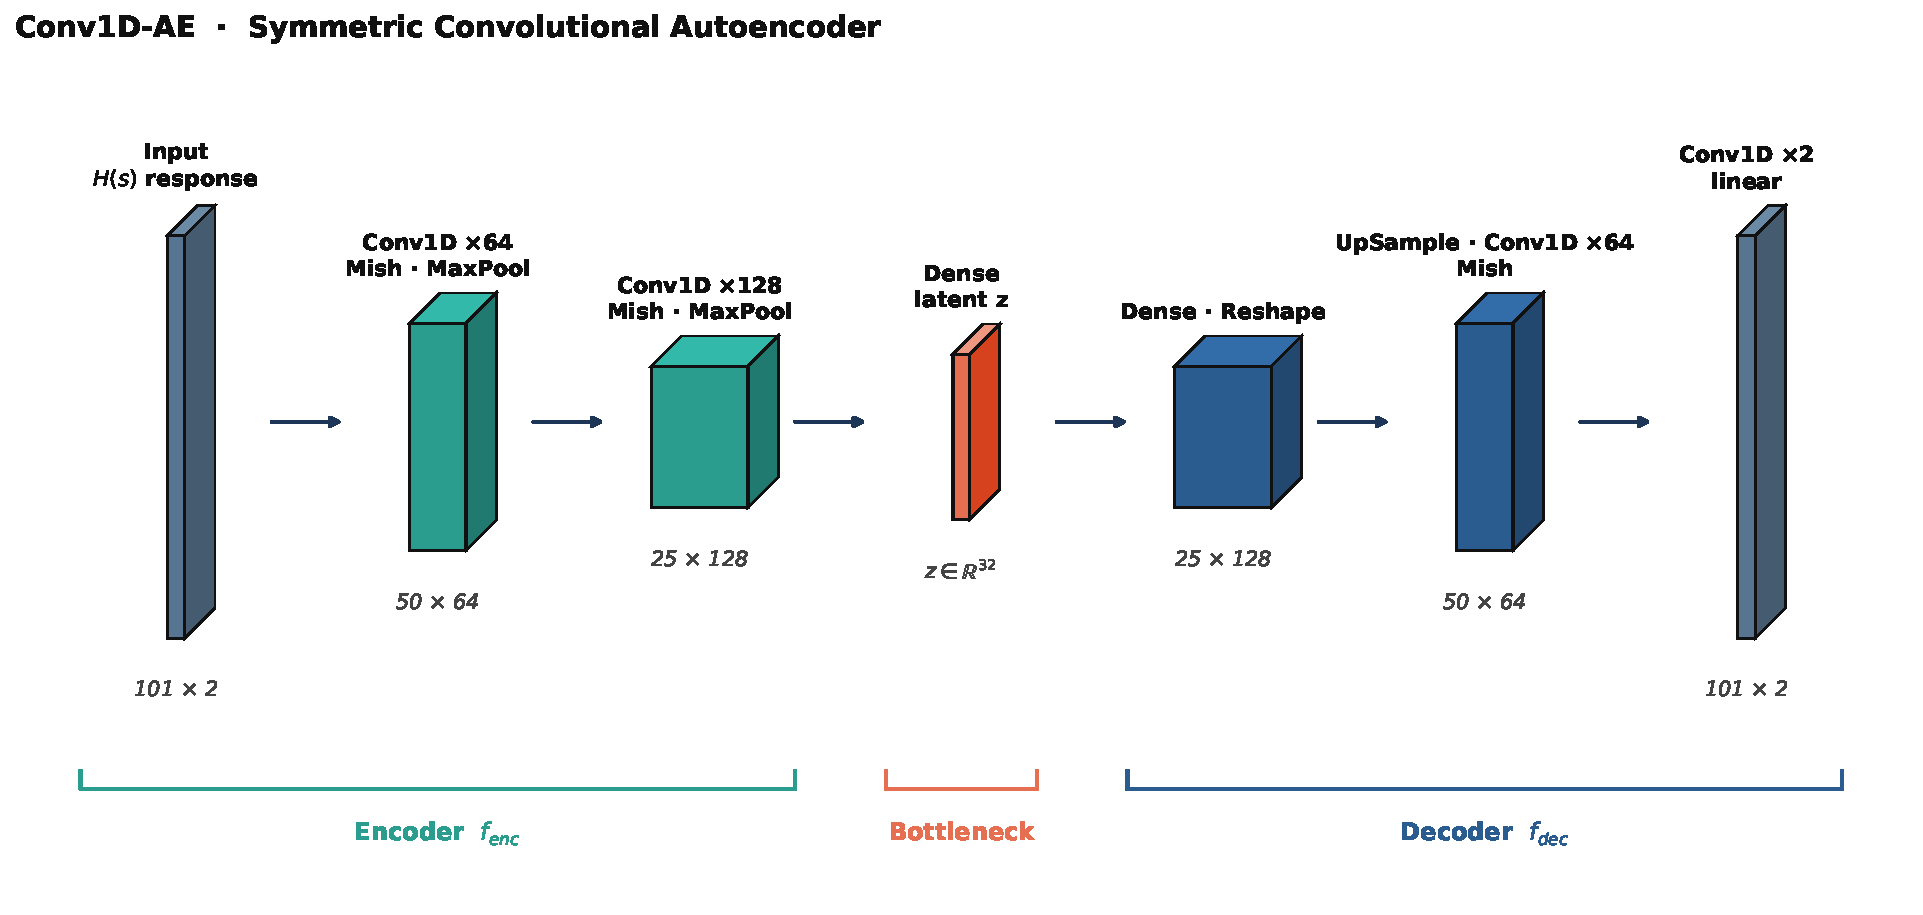
\includegraphics[width=0.82\textwidth]{arch_hero_conv1d_ae.pdf}
\caption{Conv1D-AE architecture: 1-D strided convolutional encoder with bottleneck projection and transposed-convolution reconstruction decoder.}
\label{fig:arch-conv1d}
\end{figure}

To evaluate representation capacity, we benchmark five distinct encoder families within the same self-supervised framework. Table~\ref{tab:architectures} details their architectural mechanisms and search boundaries. All models share common global hyperparameter ranges: latent dimension $d_{\mathrm{latent}} \in \{32, 64, 128, 256\}$, projection dimension $d_{\mathrm{proj}} \in \{64, 128, 256, 512\}$, and dropout rate $p_{\mathrm{drop}} \in \{0.0, 0.1\}$. Decoders are used solely during training to regularize representation learning; only the encoder backbone and projection head are retained during deployment. Fig.~\ref{fig:arch-conv1d} illustrates the Conv1D-AE baseline.

\section{Physics-Informed CARLA Contrastive Autoencoder}
\label{sec:carla}

\begin{figure}[t]
\centering
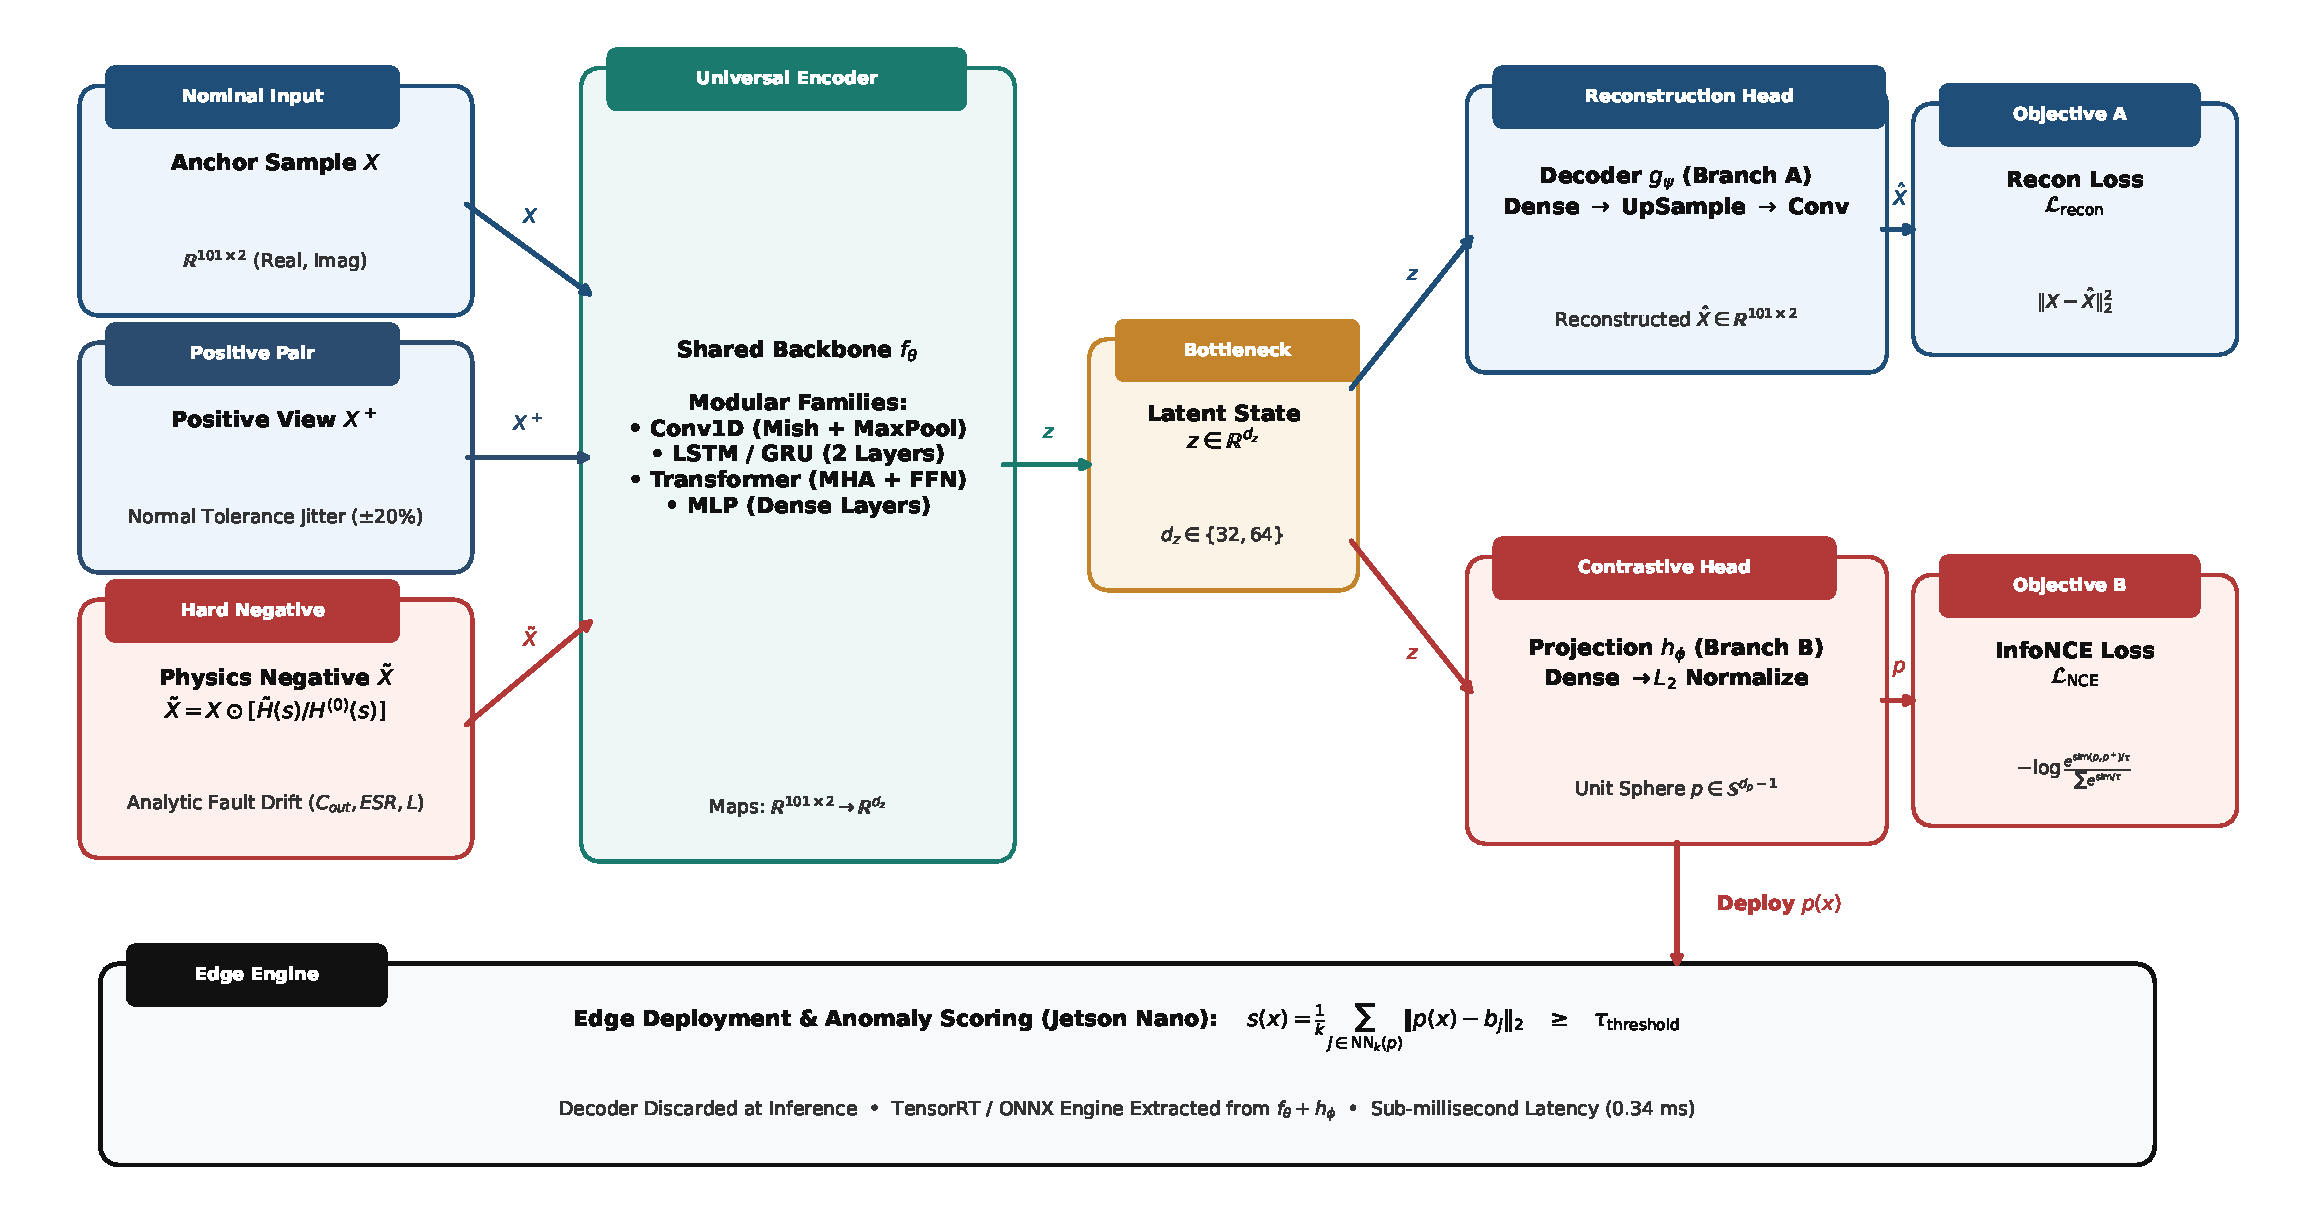
\includegraphics[width=0.95\textwidth]{arch_diagram_carla.pdf}
\caption{Physics-informed CARLA contrastive anomaly detection framework: a shared universal backbone encoder $f_{\boldsymbol{\theta}}(\cdot)$ feeds both a reconstruction decoder $h_{\boldsymbol{\psi}}(\cdot)$ and an $L_2$-normalized contrastive projection head $g_{\boldsymbol{\phi}}(\cdot)$, coupled with a non-parametric $k$-NN reference-bank scoring engine.}
\label{fig:arch-carla}
\end{figure}

\subsection{Framework Architecture}
The framework (Fig.~\ref{fig:arch-carla}) couples an encoder backbone $f_{\boldsymbol{\theta}}(\cdot)$ with two output heads:
\begin{enumerate}
    \item A multi-layer non-linear projection head $g_{\boldsymbol{\phi}}(\cdot)$ (hidden dimension 128, output dimension $d_{\mathrm{proj}}$) producing unit-normalized latent embeddings $\mathbf{z} = g_{\boldsymbol{\phi}}(f_{\boldsymbol{\theta}}(\mathbf{x})) / \|g_{\boldsymbol{\phi}}(f_{\boldsymbol{\theta}}(\mathbf{x}))\|_2$.
    \item A reconstruction decoder $h_{\boldsymbol{\psi}}(\cdot)$ mapping latent representations back to the input space $\hat{\mathbf{x}} = h_{\boldsymbol{\psi}}(f_{\boldsymbol{\theta}}(\mathbf{x})) \in \mathbb{R}^{101 \times 2}$.
\end{enumerate}

\subsection{Physics-Informed Negative Synthesis}
\label{sec:physics-negatives}
The central methodological innovation is the replacement of domain-agnostic heuristic noise with an analytic \textbf{physics-informed negative sampler}. Given an observed healthy frequency response $\mathbf{X}(j\omega)$, the sampler executes the following sequence:
\begin{enumerate}
    \item A candidate degradation state $\tilde{\boldsymbol{\theta}} \in \mathbb{R}^6$ is synthesized by perturbing one or more component entries from the nominal baseline $\boldsymbol{\theta}^{(0)}$. Perturbations are drawn across the five physical failure modes: capacitor ESR rise ($3$--$8\times$), capacitance drop ($0.3$--$0.7\times$), inductor saturation ($0.4$--$0.7\times$), winding resistance rise ($2$--$6\times$), or switch resistance degradation ($3$--$15\times R_{\mathrm{ds},\mathrm{eff}}$).
    \item The perturbed analytic small-signal transfer function $\tilde{H}(j\omega; \tilde{\boldsymbol{\theta}})$ is evaluated across the frequency grid via Eq.~\eqref{eq:gvd}--\eqref{eq:quality-factor}.
    \item The candidate negative signature $\tilde{\mathbf{X}}(j\omega)$ is synthesized by multiplying the observed healthy response $\mathbf{X}(j\omega)$ by the complex transfer ratio:
    \begin{equation}
    \tilde{\mathbf{X}}(j\omega) = \mathbf{X}(j\omega) \cdot \frac{\tilde{H}(j\omega; \tilde{\boldsymbol{\theta}})}{H^{(0)}(j\omega)}\,.
    \label{eq:transfer-ratio-augmentation}
    \end{equation}
\end{enumerate}
Because $\tilde{H}(j\omega; \tilde{\boldsymbol{\theta}})$ is evaluated on the exact continuous parameter vector $\tilde{\boldsymbol{\theta}}$, Eq.~\eqref{eq:transfer-ratio-augmentation} captures the non-linear, coupled shifts in natural resonance $\omega_0(\tilde{\boldsymbol{\theta}})$ and damping $Q(\tilde{\boldsymbol{\theta}})^{-1}$ via the closed-form rational function (\texttt{signal.freqs\_zpk} evaluation), preserving pole-zero structure and coherent magnitude-phase warps without per-sample ordinary differential equation (ODE) integration. The operation is exact within the small-signal LTI linearization; large-signal switching non-linearities beyond Eq.~\ref{eq:gvd} are not represented (see Sec.~\ref{sec:conclusion}).

\subsection{Training Objective and Theoretical Loss Formulation}
\label{sec:objective}
For each anchor instance $\mathbf{x}_i$, a lightly augmented positive sample $\mathbf{x}_i^+$ is formed via minor amplitude scaling ($\pm 1\%$), and an independent physics-informed negative sample $\mathbf{x}_i^-$ is generated via Eq.~\eqref{eq:transfer-ratio-augmentation}. Their projected normalized embeddings $(\mathbf{z}_i, \mathbf{z}_i^+, \mathbf{z}_i^-)$ are optimized using the two-logit InfoNCE objective~\cite{oord2018representation,chen2020simclr}:
\begin{equation}
\mathcal{L}_{\mathrm{NCE}} = -\frac{1}{N} \sum_{i=1}^N \log \frac{\exp\left(\mathrm{sim}(\mathbf{z}_i, \mathbf{z}_i^+) / \tau\right)}{\exp\left(\mathrm{sim}(\mathbf{z}_i, \mathbf{z}_i^+) / \tau\right) + \exp\left(\mathrm{sim}(\mathbf{z}_i, \mathbf{z}_i^-) / \tau\right)}\,,
\label{eq:ntxent}
\end{equation}
where $\mathrm{sim}(\mathbf{u}, \mathbf{v}) = \mathbf{u}^\top \mathbf{v}$ denotes cosine similarity on $L_2$-normalized vectors, and $\tau \in \{0.05, 0.07, 0.10\}$ is a temperature parameter. 

Crucially, mini-batch negative sampling (i.e., treating other normal training instances $\mathbf{x}_j$ as negatives) is strictly avoided in Eq.~\eqref{eq:ntxent}. In one-class unsupervised representation learning, repelling distinct healthy operating points shatters the nominal manifold into fragmented clusters, degrading boundary estimation~\cite{chen2023harnessing}. Standard InfoNCE with $K$ negatives yields the bound $I(X; Y) \ge \log(K) - \mathcal{L}_{\mathrm{NCE}}$ \cite{oord2018representation}; for $K=1$ this bound is vacuous ($\log 1=0$). We therefore do not claim a mutual-information guarantee for $K=1$; instead Eq.~\ref{eq:ntxent} is used as a directed discriminative margin objective that pushes representations away along genuine circuit failure trajectories rather than isotropic noise directions.

The composite training loss combines reconstruction and contrastive objectives:
\begin{equation}
\mathcal{L} = w_r \mathcal{L}_{\mathrm{recon}} + w_c \mathcal{L}_{\mathrm{NCE}}\,,
\label{eq:combined-loss}
\end{equation}
where $\mathcal{L}_{\mathrm{recon}} = \frac{1}{N} \sum_{i=1}^N \|\mathbf{x}_i - \hat{\mathbf{x}}_i\|_2^2$, with loss weights $w_r \in \{5, 10, 20\}$ and $w_c \in \{0.5, 1.0\}$ tuned on validation data. The reconstruction decoder regularizes the encoder against representation collapse, while the contrastive projection head shapes the metric geometry of the latent manifold.

\subsection{Anomaly Scoring Pipeline}
During inference, anomaly scoring is conducted non-parametrically using $k$-nearest-neighbor ($k$-NN) distance in the projection space~\cite{cover1967knn}:
\begin{equation}
s(\mathbf{x}) = \frac{1}{k} \sum_{j \in \mathrm{NN}_k(\mathbf{z}_x)} \|\mathbf{z}_x - \mathbf{z}_j\|_2\,, \qquad k \in \{1, 3, 5, 10, 20, 50\}\,,
\label{eq:knn-score}
\end{equation}
where $\mathrm{NN}_k(\mathbf{z}_x)$ denotes the index set of the $k$-nearest neighbors of query embedding $\mathbf{z}_x$ evaluated against the fixed reference bank $\mathcal{B}_{\mathrm{train}} = \{\mathbf{z}_j\}_{j=1}^{2419}$ containing all projected healthy training embeddings. The scoring metric (Euclidean $k$-NN, cosine distance, centroid distance, or regularized Mahalanobis distance), neighborhood size $k$, and decision threshold $\gamma$ (calibrated to the 70th--99.9th percentile of healthy fit-validation scores) are selected jointly to maximize the F1-score on the balanced fit-validation partition.

\section{Experimental Setup}
\label{sec:setup}

\textbf{Hyperparameter Optimization.} Each encoder architecture undergoes 50 independent trials using a guided sequential search (Keras-Tuner random search for initial exploration, then local perturbations of the top-3 completed configurations). The search spans Table~\ref{tab:architectures} plus global ranges $d_{\mathrm{latent}}\in\{32,64,128,256\}$, $d_{\mathrm{proj}}\in\{64,128,256,512\}$, $p_{\mathrm{drop}}\in\{0.0,0.1\}$, $\tau\in\{0.05,0.07,0.10\}$, $w_{r}\in\{5,10,20\}$, $w_{c}\in\{0.5,1.0\}$, and $k\in\{1,3,5,10,20,50\}$ for the scorer. Model training uses Adam optimization, batch size 128, maximum 30 epochs, and early stopping with patience 10 on validation loss. Pseudo-random number generator states are systematically initialized across trials to ensure reproducibility across hardware platforms. The best configuration per family is selected by fit-validation ROC-AUC~\cite{fawcett2006roc} and retrained for up to 150 epochs with early stopping patience of 20 epochs.

\textbf{Hardware Testbed.} Gradient training and architecture searches are conducted on a workstation equipped with an NVIDIA RTX~4070 GPU. Checkpoints, reference banks, and preprocessing scalers are transferred to an NVIDIA Jetson Nano edge platform (quad-core ARM Cortex-A57 CPU, 128-core Maxwell GPU, 4 GB unified LPDDR4 memory), where scorer selection and test-set inferences are physically executed.

\textbf{Evaluation Protocol.} Test performance is evaluated on the 1,268 held-out test states using accuracy, precision, recall, F1-score, ROC-AUC, and PR-AUC. Non-parametric bootstrap confidence intervals (95\% CI) are computed over 2,000 stratified resamples.

\section{Results and Discussion}
\label{sec:results}

\subsection{Encoder Family Benchmark}

\begin{table}[t]
\centering
\small
\caption{Measured test-set performance across the five evaluated encoder families on Jetson Nano ($n=1{,}268$; 520 healthy and 748 anomalous states).}
\label{tab:main-results}
\begin{tabular}{@{}lcccccc@{}}
\toprule
Model Architecture & Accuracy & Precision & Recall & F1-Score & ROC-AUC & PR-AUC \\
\midrule
CARLA--GRU & 0.8139 & 0.9444 & 0.7273 & 0.8218 & 0.8678 & 0.9290 \\
CARLA--LSTM & 0.8344 & 0.9483 & 0.7607 & 0.8442 & 0.8834 & 0.9385 \\
CARLA--Transformer & 0.8707 & 0.9650 & 0.8102 & 0.8808 & 0.9100 & 0.9538 \\
CARLA--MLP & 0.8707 & 0.9591 & \textbf{0.8155} & 0.8815 & \textbf{0.9161} & 0.9563 \\
\textbf{CARLA--Conv1D} & \textbf{0.8809} & \textbf{0.9807} & 0.8142 & \textbf{0.8897} & 0.9157 & \textbf{0.9570} \\
\bottomrule
\end{tabular}
\end{table}

\begin{figure}[t]
\centering
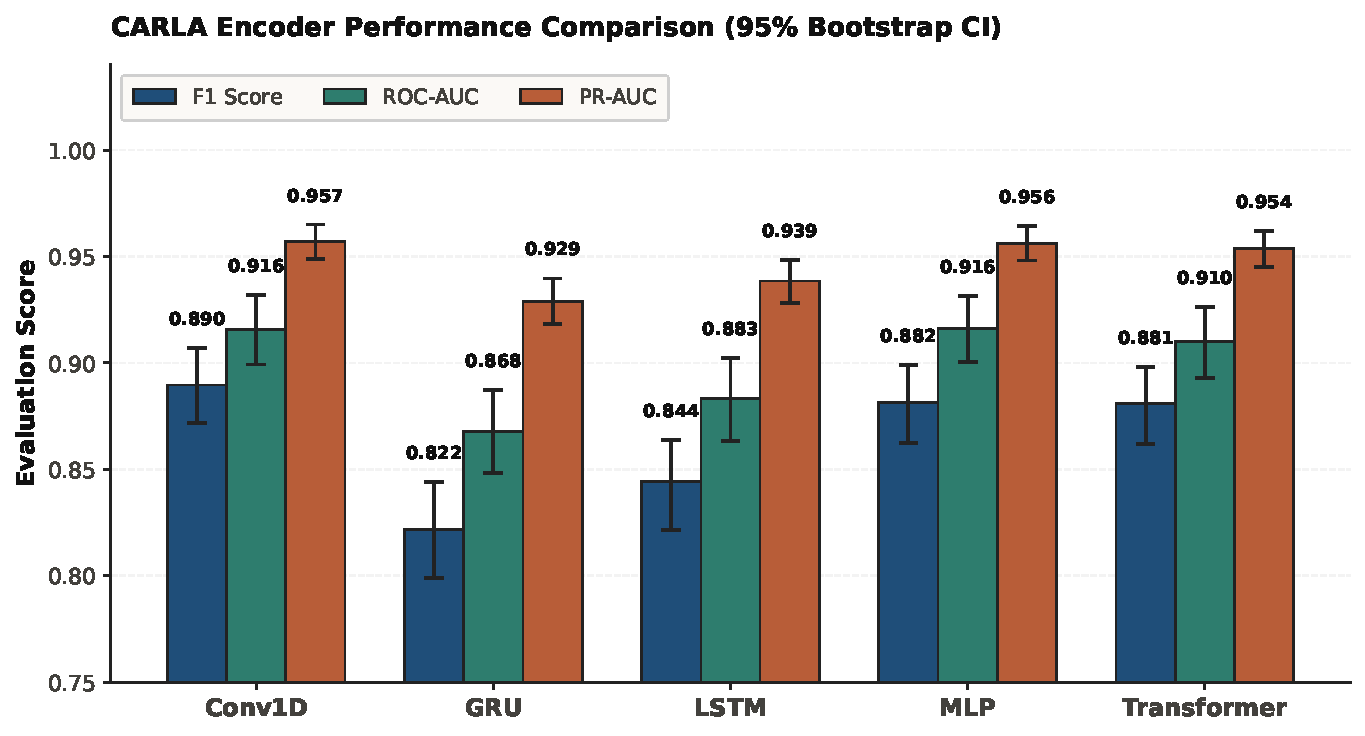
\includegraphics[width=0.88\textwidth]{latest_carla_metrics.pdf}
\caption{Measured F1-score, ROC-AUC, and PR-AUC across the five evaluated encoder families. The vertical axis is truncated to $[0.80,0.96]$ (full $[0,1]$ in inset, if space permits) to highlight the separation between convolutional/dense backbones and recurrent models; absolute scores are in Table~\ref{tab:main-results}.}
\label{fig:latest-carla-metrics}
\end{figure}

Table~\ref{tab:main-results} and Fig.~\ref{fig:latest-carla-metrics} report the comparative performance across all five encoder backbones. Conv1D achieves the highest overall classification performance with an F1-score of 0.8897, an accuracy of 0.8809, and a PR-AUC of 0.9570. MLP achieves a comparable ROC-AUC of 0.9161 (+0.0004 over Conv1D) and the highest recall (0.8155), but incurs more false positives (23 vs. 12 for Conv1D), resulting in a lower precision (0.9591 vs. 0.9807) and F1-score (0.8815).

The performance parity between Conv1D and MLP reflects the mathematical structure of the input space. On a fixed, discrete logarithmic frequency grid ($N_f = 101$), each frequency bin $f_k$ corresponds to a fixed physical coordinate rather than an arbitrary translation-invariant time step. An MLP architecture treats each frequency coordinate with independent synaptic weights, capturing global spectral relationships directly. Conv1D complements this by sharing local kernels across neighboring frequency bins, efficiently capturing local slope gradients $\frac{d|G|}{d\log f}$ and phase transitions $\frac{d\angle G}{d\log f}$ associated with resonant displacement $\Delta f_0$.

Conversely, recurrent architectures (GRU and LSTM) exhibit substantially lower recall ($0.7273$ and $0.7607$) and incur 31--32 false positives, yielding lower F1-scores ($0.8218$ and $0.8442$). Recurrent networks enforce an artificial unidirectional Markovian causality ($f_1 \to f_2 \to \dots \to f_{101}$), which imposes an unnatural directional inductive bias on static, steady-state frequency transfer functions.

\subsection{Physics-Informed Negative Sampler Ablation}

\begin{table}[t]
\centering
\small
\caption{Paired Conv1D negative-sampler ablation across three independent random weight initializations. Metrics represent mean $\pm$ sample standard deviation; initial network weights are byte-identical within each paired run.}
\label{tab:negative-sampler-ablation}
\begin{tabular}{@{}lcccccc@{}}
\toprule
Sampler Mode & Accuracy & Precision & Recall & F1-Score & ROC-AUC & PR-AUC \\
\midrule
Physics-Informed & $0.8704 \pm 0.0039$ & $0.9361 \pm 0.0133$ & $0.8378 \pm 0.0196$ & $0.8840 \pm 0.0054$ & $0.9200 \pm 0.0015$ & $0.9580 \pm 0.0012$ \\
Heuristic & $0.8533 \pm 0.0150$ & $0.9390 \pm 0.0186$ & $0.8039 \pm 0.0282$ & $0.8659 \pm 0.0154$ & $0.9180 \pm 0.0046$ & $0.9545 \pm 0.0030$ \\
\midrule
Paired Difference & $+0.0171$ & $-0.0029$ & $+0.0339$ & $+0.0181$ & $+0.0020$ & $+0.0035$ \\
\bottomrule
\end{tabular}
\end{table}

\begin{figure}[t]
\centering
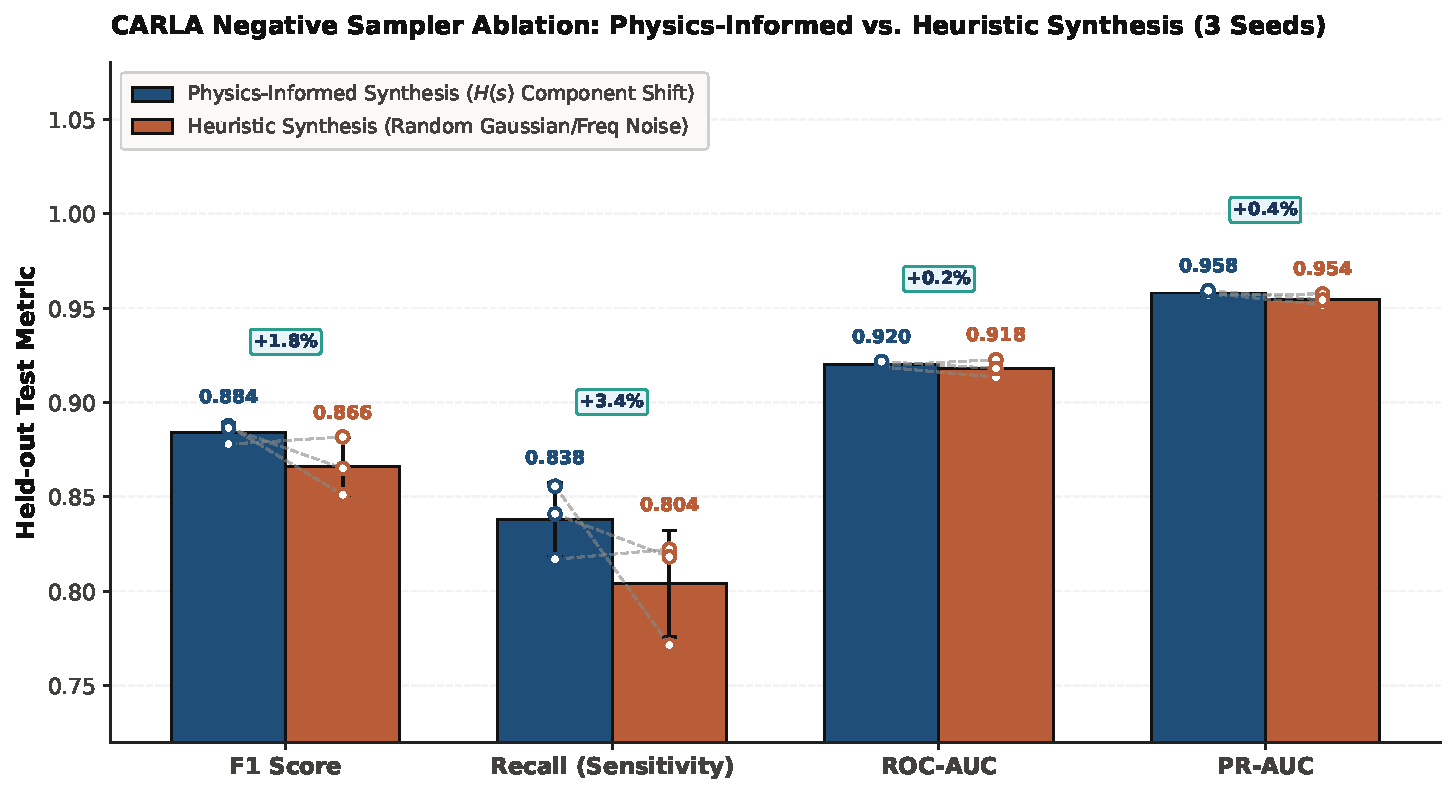
\includegraphics[width=0.78\textwidth]{negative_sampler_ablation.pdf}
\caption{Paired ablation between physics-informed and heuristic negative synthesis across three independent random initializations with byte-identical starting weights. Error bars are $\pm1$ sample standard deviation ($n=3$); per-seed F1 deltas are $+0.0366$, $-0.0038$, $+0.0215$. With $n=3$ no formal significance test is powered; the consistent positive mean is reported descriptively.}
\label{fig:negative-sampler-ablation}
\end{figure}

To isolate the contribution of physics-informed negative synthesis, we perform a controlled ablation on the optimal Conv1D architecture. Models are trained under identical conditions using either the physics-informed transfer-ratio sampler or a baseline heuristic injector (combining spectral noise, random amplitude scaling, and frequency warping). The experiment is replicated across three independent paired initializations, verifying matching SHA-256 weight hashes at initialization.

As detailed in Table~\ref{tab:negative-sampler-ablation} and Fig.~\ref{fig:negative-sampler-ablation}, physics-informed synthesis increases mean F1-score from $0.8659 \pm 0.0154$ to $0.8840 \pm 0.0054$, representing a mean paired improvement of $+0.0181$. Individual paired F1 differences across the three runs are $+0.0366$, $-0.0038$, and $+0.0215$. With $n=3$, formal paired $t$-tests are underpowered and sensitive to the single negative delta; we therefore report effect size descriptively and provide per-seed deltas rather than a $p$-value. The gain is driven primarily by a $+0.0339$ increase in recall ($0.8378$ vs.~$0.8039$), while precision remains comparable ($0.9361$ vs.~$0.9390$). Bootstrap intervals for $n=3$ are unstable and omitted; the three-seed spread itself quantifies variability. 

These results demonstrate that synthesizing negatives via analytic transfer ratios forces the encoder to learn decision boundaries that align with true physical degradation paths, significantly reducing false negatives on subtle, incipient component faults.

\section{Conclusion, Scientific Limitations, and Future Work}
\label{sec:conclusion}

This paper presented a self-supervised, physics-informed contrastive anomaly detection framework for power electronic converters. By formalizing component degradation through explicit set-membership multiplier bands and synthesizing contrastive hard negatives via analytic small-signal transfer ratios, the framework avoids representation collapse without relying on unphysical noise heuristics or labeled fault data. Extensive benchmarking across five encoder architectures established Conv1D as the superior backbone (F1: 0.8897, PR-AUC: 0.9570), with three-seed paired ablations showing a mean F1 improvement of $+0.0181$ (individual deltas $+0.0366$, $-0.0038$, $+0.0215$) from physics-grounded negative synthesis; with $n=3$ this is a descriptive effect-size finding.

A companion manuscript~\cite{jsc_edge_deployment} details the edge compilation, Post-Training Quantization (PTQ), TensorRT optimization, and rail-level power characterization of these models on embedded GPU hardware. 

\subsection{Scientific Limitations and Future Research Trajectories}
While the presented framework advances physics-informed representation learning, three foundational scientific limitations motivate future research:
\begin{enumerate}
    \item \textbf{Small-Signal Linearization vs. Large-Signal Non-Linear Dynamics:} The current generative transfer ratio $\tilde{H}(s)/H^{(0)}(s)$ is derived from small-signal state-space averaging around a fixed nominal operating point. In extreme degradation or severe load transients, converters exhibit nonlinear switching phenomena, duty cycle saturation, and switching-frequency harmonics. Future work will formulate nonlinear, state-dependent perturbation ratios incorporating large-signal averaged models and continuous differential algebraic equations (DAEs) directly into the contrastive objective~\cite{raissi2019pinn}.
    \item \textbf{In-Silico Simulation vs. Physical Hardware Domain Shift:} The training and benchmark datasets are generated in high-fidelity PSIM digital twins. Physical Frequency Response Analyzer (FRA) hardware injections introduce swept-sine measurement jitter, parasitic printed circuit board (PCB) trace couplings, and sensor non-linearities. Bridging this gap will require unsupervised domain adaptation and adversarial feature alignment to transfer digital-twin representations to noisy physical instrumentation.
    \item \textbf{Topological Generalization to Multi-Converter Microgrids:} The reference implementation focuses on a single-stage buck converter. Extending the formulation to multi-input multi-output (MIMO) transfer function matrices $\mathbf{H}(s)$ will enable self-supervised anomaly detection across interleaved topologies, multi-phase inverters, and interconnected DC microgrid power distribution systems.
    \item \textbf{Emerging Neural Operator Backends:} Future investigations will explore selective state-space models such as Mamba~\cite{gu2023mamba} for long-range spectral scanning and Kolmogorov--Arnold Networks (KAN)~\cite{liu2024kan} for symbolic mathematical interpretability of the latent anomaly manifold.
\end{enumerate}

\section{Reproducibility Statement}
\label{sec:reproducibility}

The complete experimental workflow is deterministic and fully auditable. The open-source project repository (\url{https://github.com/igmsalinas/fault_converters}) provides the PSIM simulation generation scripts, deduplicated split indices, training configurations, initial-state weight verification hashes, and locked test-set evaluation records. Workstation training scripts and Jetson Nano inference runbooks are openly accessible.

\section*{Data Availability Statement}
The simulation dataset, pre-trained model weights, and generation code are openly available as an open-source contribution at \url{https://github.com/igmsalinas/fault_converters}.

\section*{Conflict of Interest Statement}
The authors declare no competing financial or non-financial interests.

\bibliographystyle{IEEEtran}
\bibliography{references}

\end{document}
